% ****** Start of file apssamp.tex ******
%
%   This file is part of the APS files in the REVTeX 4.2 distribution.
%   Version 4.2a of REVTeX, December 2014
%
%   Copyright (c) 2014 The American Physical Society.
%
%   See the REVTeX 4 README file for restrictions and more information.
%
% TeX'ing this file requires that you have AMS-LaTeX 2.0 installed
% as well as the rest of the prerequisites for REVTeX 4.2
%
% See the REVTeX 4 README file
% It also requires running BibTeX. The commands are as follows:
%
%  1)  latex apssamp.tex
%  2)  bibtex apssamp
%  3)  latex apssamp.tex
%  4)  latex apssamp.tex
%
\documentclass[%
 reprint,
%superscriptaddress,
%groupedaddress,
%unsortedaddress,
%runinaddress,
%frontmatterverbose, 
%preprint,
%preprintnumbers,
%nofootinbib,
%nobibnotes,
%bibnotes,
 amsmath,amssymb,
 aps,
%pra,
%prb,
%rmp,
%prstab,
%prstper,
%floatfix,
]{revtex4-2}

\usepackage{algorithm}
\usepackage{algorithmic}
\usepackage{graphicx}% Include figure files
\usepackage{dcolumn}% Align table columns on decimal point
\usepackage{bm}% bold math
%\usepackage{hyperref}% add hypertext capabilities
%\usepackage[mathlines]{lineno}% Enable numbering of text and display math
%\linenumbers\relax % Commence numbering lines

%\usepackage[showframe,%Uncomment any one of the following lines to test 
%%scale=0.7, marginratio={1:1, 2:3}, ignoreall,% default settings
%%text={7in,10in},centering,
%%margin=1.5in,
%%total={6.5in,8.75in}, top=1.2in, left=0.9in, includefoot,
%%height=10in,a5paper,hmargin={3cm,0.8in},
%]{geometry}
\bibliographystyle{apsrev4-1}

\begin{document}

\preprint{APS/123-QED}

\title{Qubit Routing using Graph Neural Network aided Monte Carlo Tree Search}

\author{Animesh Sinha}
\email{animesh.sinha@research.iiit.ac.in}
\author{Utkarsh Azad}
\email{utkarsh.azad@research.iiit.ac.in}
\author{Jai Bardhan}
\author{Kalp Shah}
\author{Bhuvanesh Sridharan}
\author{Dr. Harjinder Singh}
\email{laltu@iiit.ac.in}
\affiliation{%
    Center for Computational Natural Science, International Institute of Information Technology, Hyderabad.
}%

\date{\today}% It is always \today, today,
%  but any date may be explicitly specified

\begin{abstract}
    Current day Quantum Computers offer limited connectivity, two qubit operations can only be applied on physically neighboring qubits. To respect this constraint when compiling quantum circuits to some hardware, we need to insert swap gates. It's desirable that the depth of the final circuit with the inserted gates is minimized, this article aims to provide an efficient solution to this problem.

    We use Monte Carlo Tree Search to perform qubit routing, which is aided by a Graph Neural Network for evaluating the long term value of states as well as estimating prior probabilities of which actions are worth exploring. Minimizing circuit depth involves being able to perform operations in parallel, we using mutex locks to efficiently maintain this information and present it to the neural network. This should be of relevance to both the particular task of Qubit routing and as a general idea in several combinatorial optimizations.
\end{abstract}

\keywords{Qubit Routing, Quantum Compilation, Quantum Circuit Transformation, Reinforcement Learning, Monte Carlo Tree Search, Graph Neural Network}
\maketitle

%\tableofcontents

\section{\label{sec:intro}Introduction}

\subsection{\label{sec:intro-defn}Describing the Problem}

Present day quantum computer come in a variety of hardware architectures, but a pervading problem across them is limited qubit connectivity for two qubit operations and high error rates, which compound when increasing the depth of the circuit, due to which the execution of deep quantum circuits is an unfeasible task.

To make an arbitrary quantum circuit executable on a given target architecture, a quantum compiler has to insert SWAP gates so that gates in the original circuit only ever occur between qubits located at adjacent nodes, a process known as Qubit Routing. The process produce a new circuit, possibly with a greater depth, that implements the same unitary function as the original circuit while respecting
the topological constraints \citep{qroute_dqn2}.

\begin{figure}
    \centering
    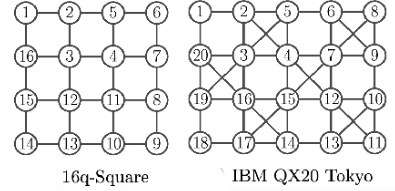
\includegraphics[width=\linewidth]{images/topology-graph.png}
    \caption{Topology for Common Device Architectures \citep{photo_architecture_graph}}
    \label{fig:topology-example}
\end{figure}

Minimizing the depth of the quantum circuit resulting from the routing process is the objective we are trying to achieve.


\subsection{\label{sec:intro-related}Related Work}

The problem of Qubit routing was outlined and presented with a graph based architecture-agnostic solution by \citet{qroute_tket}. The routing problem was phrased as a reinforcement learning problem in a combinatorial action space by \citet{qroute_dqn1}. They also proposed the use of simulated annealing to search through the combinatorial action space, aided by a Feed Forward Neural Network to judge the long-term expected compilation time. This was extended to use Double Deep Q-learning and Prioritized Experience Replay by \citet{qroute_dqn2}.

Monte Carlo Tree Search (MCTS) has been a popular reinforcement learning algorithm \citep{mcts_bandits_0, mcts_bandits_1, mcts_uct} leading to great success in a variety of domains, playing puzzle games like Chess and Go \citep{mcts_alphago} for instance.
A version of MCTS, adapted for better exploration on Asymmetric Trees was proposed by \citet{mcts_assymetric}, which will be the formulation of choice for us.
An unaided Monte Carlo Tree Search in the context of minimizing the total volume of quantum circuits (number of gates, ignoring the parallelization) was proposed by \citet{qroute_mcts}, and has produced promising results.

\subsection{\label{sec:intro-contribution}Contribution of this work}

This article proposes using Monte Carlo tree search for the task of total Depth minimization, as an easier to train and better performing machine learning setting.
\begin{itemize}
    \item We use an array of mutex locks to represent the information the Agent needs to know to be able to make effective use of parallelization.
    \item We propose a graph neural network architecture to approximate the value function and the policy function for any given state of the system.
    \item We provide a simple python package to test and visualize routing algorithms with different neural net architectures, combining algorithms, reward structures, etc.
\end{itemize}
From these changes, we hope to gain an agent which is not immediately greedy since it can only see the current state and not effectively plan for the future, and to stabilize the decision process which suffered from the randomness of introduced by simulated annealing.


\section{\label{sec:method}Method}

The solution to this problem involves maintaining a convenient representation of the current state of the total system, that is the remainder of the problem and the current state of the solution, and evolving it using actions chosen by our model. In this section we describe both these steps. (Code for the complete simulation and visualization is available on \url{https://github.com/AnimeshSinha1309/quantum-rl})

\subsection{\label{sec:method-state}State representation}

\subsubsection{\label{sec:method-state-circuit}Circuit Representation}

Each circuit is input as a set of qubit $\mathbb{Q}$ and an partially ordered set of operations $\mathbb{O} = \{(q_x, q_y) \vert q_x, q_y \in \mathbb{Q}\}$.
We convert this to a lists of lists representation as in \citet{qroute_dqn2}, where for each logical qubit, $q_i$, we store the list of all other qubits that participate in 2 qubit operations with $q_i$, in the order they appear in the logical circuit.

\label{para:method-state-circuit-gatecond}So a gate $(q_x, q_y)$ is executable if and only if the first $i - 1$ operations for $q_x$ and $j - 1$ operations for $q_y$ have been executed and the $i^{th}$ operation for $q_x$ is $q_y$ and the $j^{th}$ operation for $q_y$ is $q_x$.

\subsubsection{\label{sec:method-state-mutex}Mutex Locks}

The core of the routing problem lies in the parallelization of the actions under the constraints that two operations in the same timestep cannot operate on the same qubit. A way to think about this is to call the qubits "resources" and the operations that are trying to use the "consumers" of this resource. This is reminiscent of several parallel processes competing for the same memory. We try to adapt the same solution of mutual exclusions locks \citep{mutex_dijkstra} in this version of the problem.

Our output circuit will consist of 2 types of operations, CNOTs and SWAPs. All single qubit operations are much faster than any 2 qubit operations and therefore ignored. Depending on the primitive gates available on the hardware, a SWAP can either be an elementary gate and equivalent to CNOT, or be decomposed into 3 CNOT gates. So the locks array, which is a part of the state, should be a vector $l_t \in Z_+^{n_nodes}$. For each of the nodes, it states the number of timesteps it will stay locked for. This vector is also presented to the Neural Network so help it learn to avoid attempting to use the same node and several operations.

\subsubsection{\label{sec:method-state-full}The State Object}

Our simulation will proceed in timesteps. The entire specification of our system will be done by the state $s_t = (C, D, q_t, p_t, l_t)$.
\begin{itemize}
    \item $q_t \in \mathbb{Z}^{n\_nodes}_{n\_nodes}$ is a vector denoting the qubit locations, the i\textsuperscript{th} element in the array denotes the index of the logical qubit which is present on the i\textsuperscript{th} element.
    \item $p_t \in \mathbb{Z}^{n\_nodes}_{+}$ is a vector which represents the progress of each qubit on the circuit.
    \item $l_t \in \mathbb{Z}^{n\_nodes}_{+}$ is a vector which stores the number of operations this qubit will stay locked for. It's a mutex lock of sorts, ensuring that a CNOT operation blocks a qubit for the next timestep, or a swap gate blocks it for the next 3.
    \item $C$ - the circuit object. Common across all states, contains the list of lists representation of the circuit.
    \item $D$ - the device object. Allows access to the shortest distance between any two nodes on the device graph, thereby also checking if a two qubit gate is admissible on the hardware given the nodes it has to operate on.
\end{itemize}

\subsubsection{\label{sec:method-state-actions}Action Space}

Through our search, we evolve the state using Actions. These actions are one of two types: $SWAP(a, b)$ or $CNOT(a, b)$. A $SWAP$ action evolves the mapping by swapping elements in the qubit locations array $q_t$. A $CNOT$ action is only performed when a gate in the logical circuit is executable, as described here (\ref{para:method-state-circuit-gatecond}), and satisfies the topological constraints of the circuit.

\subsection{\label{sec:method-rl}Reinforcement Learning Setting}

Given a state $s$, the value function of that state is the expected total reward in the future.
\begin{equation}
    V(s) = \max_{s^\prime} Q(s, a)
\end{equation}

The Q-function is the total expected reward in the future after we took an action A from state S. This is updated in each step of our simulation for all the states that were visited.
\begin{equation}
    Q(s, a) = \sum_{s^\prime} R(s, a, s^\prime) + \gamma V(s^\prime)
\end{equation}

We want to find the $a$, for each $s$ which maximizes $Q(s, a)$, however, since we have to approximate $Q(s, a)$ by explicitly trying out all A, we employ a tree search to maximize this function.

\subsection{\label{sec:method-mcts}Monte Carlo Tree Search}

\begin{figure}[H]
    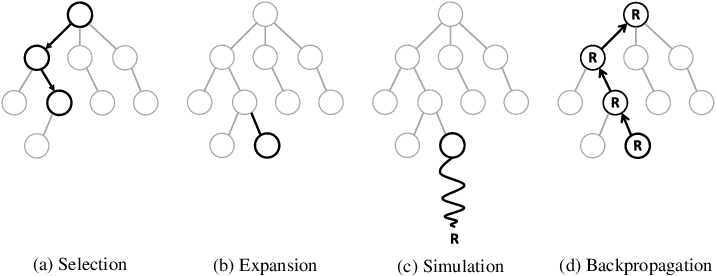
\includegraphics[width=\linewidth]{images/mcts-explainer.jpg}
    \caption{\label{fig:mcts-explainer}
        Scaling of Initial Depth overhead with size of hardware}
\end{figure}

\begin{equation}
    UCT_s(a) = Q(s, a) + \sqrt{\frac{n(s, a)}{1 + n(a)}} \times p(s, a)
\end{equation}

We recognize that running MCTS on this problem results in a highly assymetric tree, since some actions block a lot of other actions, and some actions don't interfere with any other action at all. So we add a Dirichlet noise term in the prior generated by our neural network to prevent our tree search from getting stuck down a single path. The formulation of MCTS for asymmetric trees is adapted from \citet{mcts_assymetric}

\subsection{\label{sec:method-architecture}Neural Network Architecture}

Our tree search needs a value function approximator and a policy function approximator. The Value function will help us evaluate the total expected rewards from a state. The policy function will help choose which actions are with exploring. It's seems easier to learn a good policy function, since it's heavily dependent only on the current state, as opposed to a value function which depends a lot on the expected rewards in the future.

is a neural network which helps approximate the value function, which is an estimate of the number of additional timesteps that the circuit might take to compile, and the policy function, which is a vector of size $n\_edges$, with real valued elements between 0 and 1.

\begin{figure*}[t]
    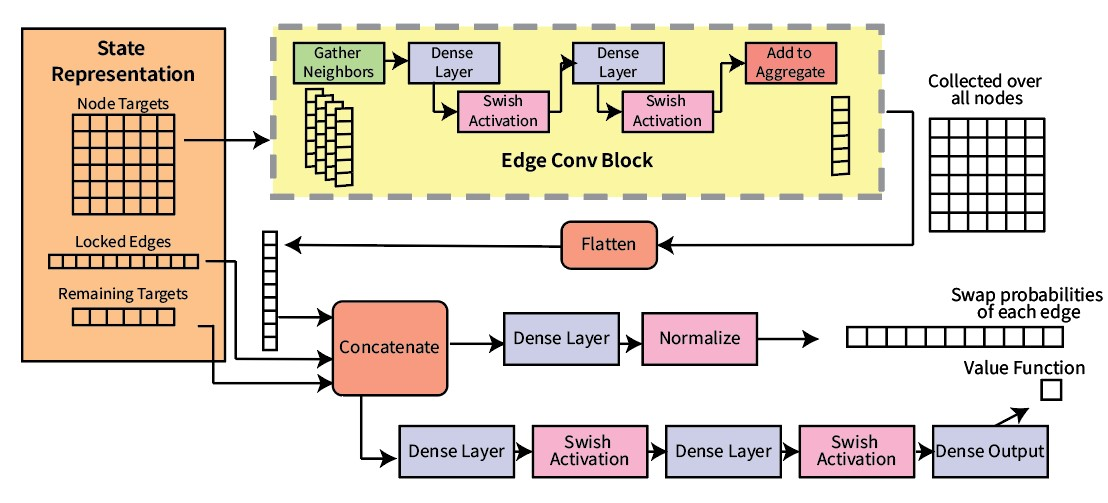
\includegraphics[width=\textwidth]{images/network-architecture.jpg}
    \caption{\label{fig:network-architecture}
        Graph Neural Network Architecture with a Value head and a Policy head}
\end{figure*}


\section{\label{sec:results}Results}

\subsection{\label{sec:results-full}Full Layer Circuits}

A full layer in a quantum circuit refers to a logical circuit that has operations on all qubits such that each qubit is involved in exactly one operation. Such a circuit is perfectly parallelizable and can be executed in a single step. Therefore is serves as a test for the initial mapping as well as a sanity check for the parallelization step.

Given a good initial mapping, we manage to transform the circuit with no depth overhead. The results for our default algorithm (Not made specifically for this task, are shown in the graph \ref{fig:results-full})

\begin{figure}[H]
    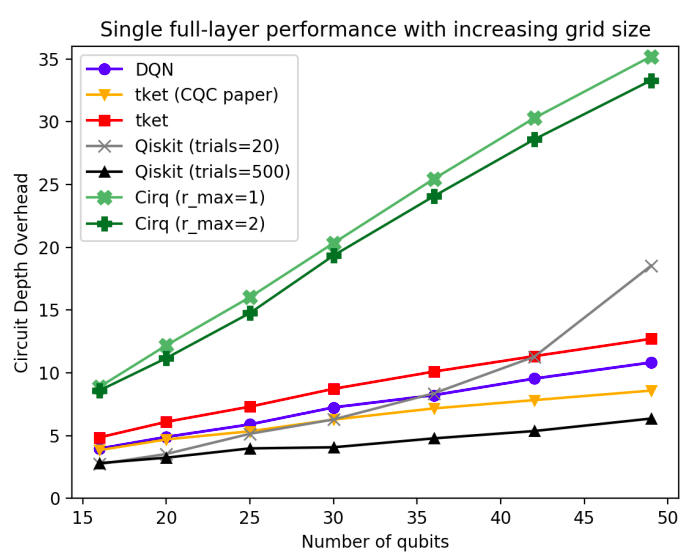
\includegraphics[width=\linewidth]{images/results-full.png}
    \caption{\label{fig:results-full}
        Scaling of Initial Depth overhead with size of hardware}
\end{figure}

\subsection{\label{sec:results-random}Random Test Circuits}

\begin{figure}[H]
    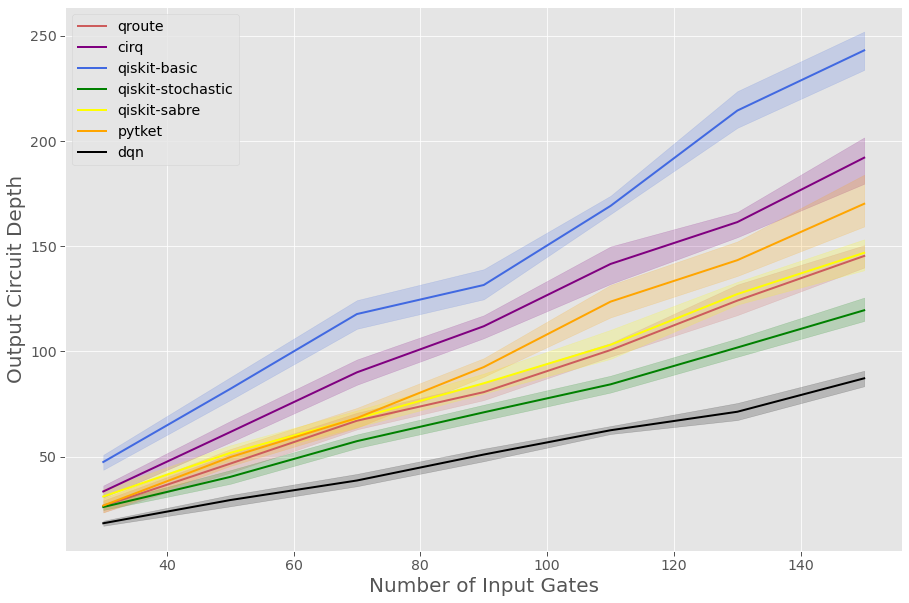
\includegraphics[width=\linewidth]{images/results-random.png}
    \caption{\label{fig:results-random}
        Depth overhead on random circuits against number of gates in input circuit and number of qubits in the hardware.}
\end{figure}

\begin{figure}[H]
    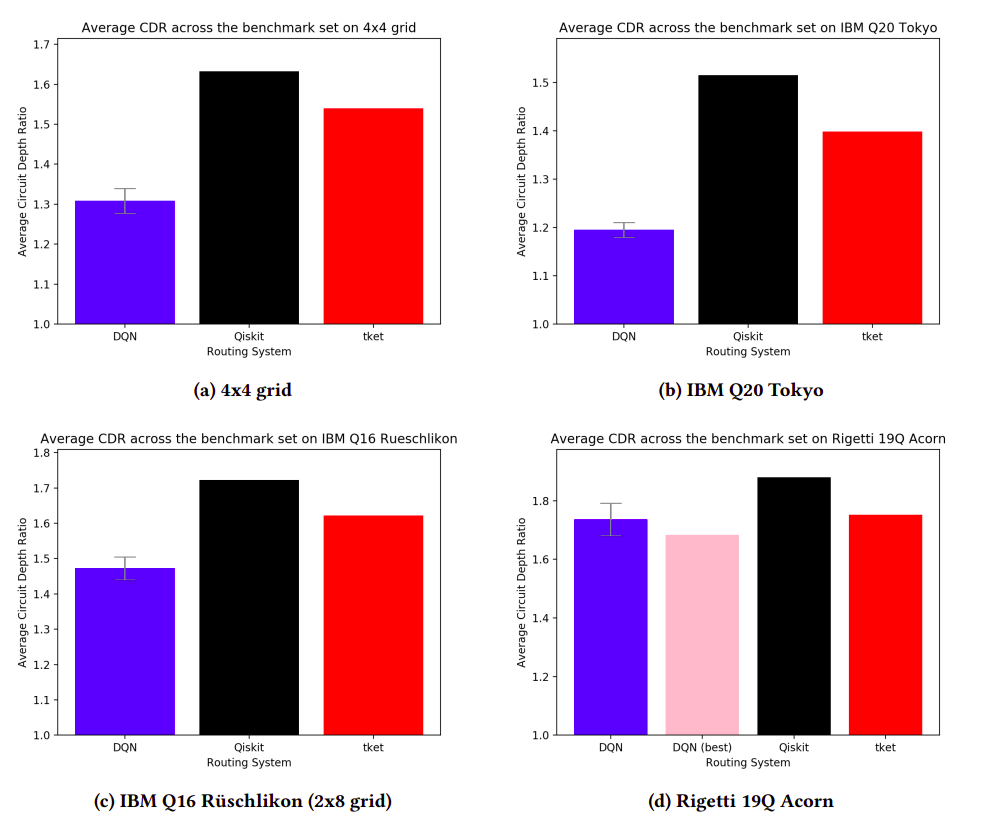
\includegraphics[width=\linewidth]{images/results-hardwares.png}
    \caption{\label{fig:results-hardware}
        Comparative performance against other methods across real world hardware}
\end{figure}


\subsection{\label{sec:results-realistic}Realistic Test Set}

\begin{table}[H]
    \caption{\label{tab:small-circuits}%
        Results of our algorithm on a set of realistic test circuits
    }
    \begin{ruledtabular}
        \begin{tabular}{lrrr}
            \textrm{Circuit}        &
            \textrm{Gate Count}     &
            \textrm{Cirq Depth}     &
            \textrm{MCTS Depth}                 \\
            \colrule

            \verb+rd84_142+  & 154  &  & \\
            \verb+adr4_197+  & 1498 &  & \\
            \verb+radd_250+  & 1405 &  & \\
            \verb+z4_268+  & 1343 &  & \\
            \verb+sym6_145+  & 1701 &  & \\
            \verb+misex1_241+  & 2100 &  & \\
            \verb+rd73_252+  & 2319 &  & \\
            \verb+cycle10_2_110+  & 2648 &  & \\
            \verb+square_root_7+  & 3089 &  & \\
            \verb+sqn_258+ & 4459 &  & \\
            \verb+rd84_253+ & 5960 &  & \\
        \end{tabular}
    \end{ruledtabular}
\end{table}


\begin{table}[H]
    \caption{\label{tab:large-circuits}%
        Results of our algorithm on a set of realistic test circuits
    }
    \begin{ruledtabular}
        \begin{tabular}{lrrr}
            \textrm{Circuit}        &
            \textrm{Gate Count}     &
            \textrm{Cirq Depth}     &
            \textrm{MCTS Depth}                 \\
            \colrule

            \verb+rd84_142+ & 154  &  & \\
            \verb+adr4_197+ & 1498 &  & \\
            \verb+radd_250+ & 1405 &  & \\
            \verb+z4_268+ & 1343 &  & \\
            \verb+sym6_145+ & 1701 &  & \\
            \verb+misex1_241+ & 2100 &  & \\
            \verb+rd73_252+ & 2319 &  & \\
            \verb+cycle10_2_110+ & 2648 &  & \\
            \verb+square_root_7+ & 3089 &  & \\
            \verb+sqn_258+ & 4459 &  & \\
            \verb+rd84_253+ & 5960 &  & \\
        \end{tabular}
    \end{ruledtabular}
\end{table}

\subsection{\label{sec:results-full}Full Layer Circuits}

Since we always greedily enqueue all operations that are executable, the depth overhead due to the routing algorithm is non-existant, we never try to introduce any swaps. This just gives us a test of our initial mapping method and provides a sanity check.

\subsection{\label{sec:results-rnd}Randomized Circuit}

We test the scaling of our algorithms on randomized circuits of varying lenghts as

\subsection{\label{sec:results-rnd}Speed of Transformation Process}

Our Method is significantly faster than all other classical methods while still producing decent results. All our large circuit benchmarks are with 100 MCTS runs per step. The Following Image shows the time taken by our algorithm and Cirq. We do not have this for over 2000 gates since Cirq didn't manage to output a result in over 2 days.

\begin{figure}[H]
    \centering
    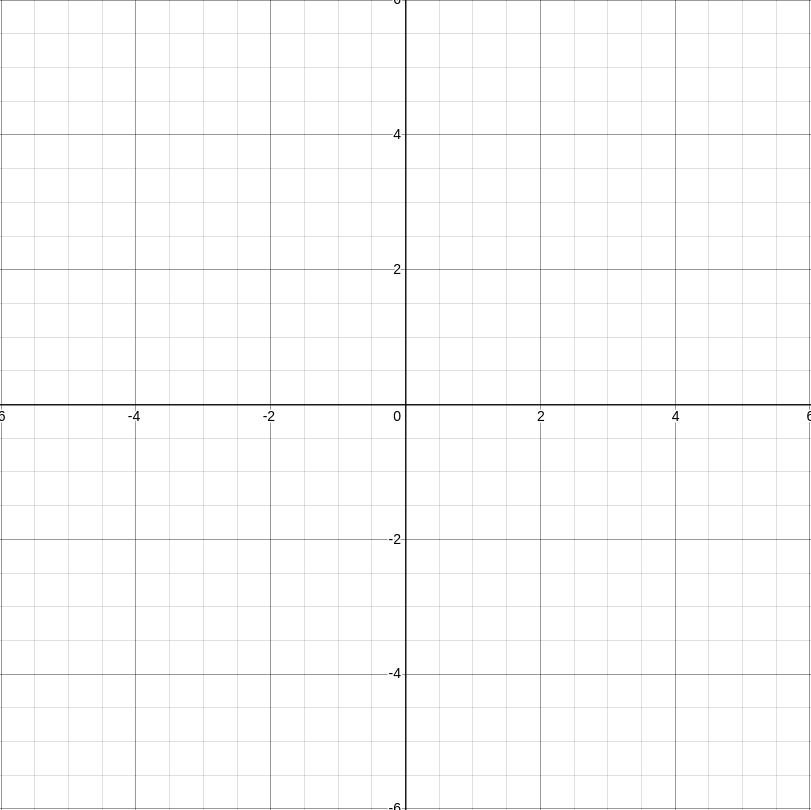
\includegraphics[width=0.6\linewidth]{images/dummy_plot.png}
    \caption{Time Taken as a function of Circuit Size}
    \label{fig:results-time}
\end{figure}

\section{Discussion and Future Scope}

However, this is my no means a definitive solution to the task of Quantum Circuit Transformations, and offers great scope of improvement. We believe that the following are avenues in which

\appendix

\section{Visualization Library}

Along with the method, we also provide a visualization library written using the Manim library for Grid Architectures.

\subsection{\label{sec:method-mcts}Monte Carlo Tree Search}

This is the basic structure of a generic Monte Carlo Tree Search algorithm aided by a value network and a policy network \citep{mcts_alphago}.

\begin{algorithm}[H]
    \caption{Monte Carlo Tree Search}
    \label{algmcts}
    \begin{algorithmic}
        \STATE {\bfseries Input:} state $s_i$, model $m$

        \sbox0{$\vcenter{\hbox{$\begin{array}{|c|c|c|} \hline 0 & \ldots & 0 \\ \hline\end{array}$}}$}
        answer $\leftarrow \underbrace{\vrule width0pt depth \dimexpr\dp0 + .3ex\relax\copy0}_{\textrm{|device.edges|}}$

        \STATE Initialize $root \leftarrow$ Node($s_i$, answer)

        \FOR{$i$ \bf{in} range $n\_mcts$}
        \STATE set $state \leftarrow$ root
        \REPEAT
        \STATE select($state$, $model$) $\rightarrow action$
        \IF{$state.child[action] \neq null$}
        \STATE $action\_type \leftarrow selection$
        \STATE $state \leftarrow state.child[action]$
        \ELSE
        \STATE $action\_type \leftarrow expansion$
        \STATE expand ($state$, $action$)
        \ENDIF
        \UNTIL{$action\_type = expansion$}
        \STATE rollout($state$) $\rightarrow reward$
        \STATE backup($state$, $reward$) $\rightarrow m$
        \ENDFOR
    \end{algorithmic}
\end{algorithm}

We recognize that running MCTS on this problem results in a highly assymetric tree, since some actions block a lot of other actions, and some actions don't interfere with any other action at all. So we add a Dirichlet noise term to prevent our tree search from getting stuck down a single path. \citep{mcts_assymetric}

\begin{algorithm}[H]
    \caption{Selection Algorithm}
    \begin{algorithmic}
        \STATE {\bfseries Input:} MCTS tree node $state$, model $m$
        \STATE $prior \leftarrow m(state) + dirichlet$
        \STATE Compute $UCT_i \leftarrow q_i + c \times \sqrt{\frac{n_i}{1 + \sum n_i}} \times prior$ $\forall i$
        \STATE Choose node $i$ with max $UCT_i$, randomly breaking tie
    \end{algorithmic}
\end{algorithm}

\begin{algorithm}[H]
    \caption{Expansion Algorithm}
    \begin{algorithmic}
        \STATE {\bfseries Input:} MCTS tree node $state$, action $a$
        \IF{a = commit}
        \STATE $new\_action$ $\leftarrow$ vector with all 0s.
        \STATE $step\_reward \leftarrow 0$
        \ELSE
        \STATE $new\_action$ $\leftarrow$ copy of $state.action$ with $a^{th}$ element set to 1.
        \STATE $step\_reward \leftarrow 0$
        \ENDIF
        \STATE $state.child[a] \rightarrow$ new node ($action$, $step\_reward$)
    \end{algorithmic}
\end{algorithm}

\begin{algorithm}[H]
    \caption{Rollout Algorithm}
    \begin{algorithmic}
        \STATE {\bfseries Input:} MCTS tree node $state$, model $m$
        \STATE $next\_state \leftarrow$ environment step ($state$)
        \RETURN $m(next\_state)$
    \end{algorithmic}
\end{algorithm}

\begin{algorithm}[H]
    \caption{Backup Process}
    \begin{algorithmic}
        \STATE {\bfseries Input:} MCTS tree node $state$, model $m$
        \STATE $prior \leftarrow m(state) + dirichlet$
        \STATE Compute $UCT_i \leftarrow q_i + c \times \sqrt{\frac{n_i}{1 + \sum n_i}} \times prior$ $\forall i$
        \STATE Choose node $i$ with max $UCT_i$, randomly breaking tie
    \end{algorithmic}
\end{algorithm}

\nocite{*}

\bibliography{qroute}% Produces the bibliography via BibTeX.

\end{document}
%
% ****** End of file apssamp.tex ******
